\chapter{مرور پیشینه پروژه}\label{ch:rl}

\section{مقدمه‌ای در مورد ماشین های خودران}
\subsection{اتومبیل‌های خودران چگونه حرکت می‌کنند؟}
 ایلان ماسک، موسس و مدیرعامل شرکت خودروسازی تسلا وعده داده که اتومبیل های خودران این شرکت از سال 2020 میلادی وارد بازار می شوند، شرکت ژاپنی نیسان اعلام کرده که اتومبیل های نیمه خودران این شرکت تا سال 2020 آماده فروش می شوند و گوگل نیز چند سالی است که سرگرم آزمایش خودروی بدون راننده خود است.

ایده رانندگی خودکار و بدون نیاز به راننده شاید چندان جدید نباشد، چرا که از سال ها پیش با آن در فیلم های علمی تخیلی آشنا شده ایم. اما هدفی که شرکت های خودروسازی امروزه دنبال می کنند، تحقق بخشیدن به این رویا است. اما از آنجایی که این فناوری هنوز در مراحل ابتدایی خود است و کمتر کسی را پیدا می کنید که از طرز کار خودروهای خودران آگاهی داشته باشد.







\subsection{اتومبیل های خودران در یک نگاه}

اتومبیل های خودران قادر هستند تا بدون دخالت عامل انسانی، رویدادهای محیط پیرامون خود را حس کنند و به حرکت درآیند. به این منظور، اتومبیل های خودران معمولا دارای یک تراشه موقعیت یابی یا \lr{GPS}، یک سیستم ناوبری اینرسی و مجموعه ای از حسگرها هستند که از میان آنها می توان به حسگرهای لیزری فاصله یاب، راداری و ویدیویی اشاره کرد. خودرو در واقع از اطلاعات موقعیتی فراهم شده از سوی ماهواره های \lr{GPS} و سیستم ناوبری اینرسی برای تشخیص موقعیت خود، و از اطلاعات حسگرها برای شناسایی جهت و جزییات محیط اطرافش استفاده می کند و در نهایت تصویری سه بعدی از محل کنونی خود و محیط پیرامون خود تهیه می کند.

طی این فرایند، اطلاعات بدست آمده از هر حسگر فیلتر می شود تا نویزهای آن حذف شود و سپس با یکدیگر ترکیب می شوند تا تصویر نهایی تولید شود. حال نوبت به سیستم کنترل خودرو می رسد تا براساس این تصویر، نسبت به تعیین مسیر و سایر موارد مرتبط با هدایت خودرو تصمیم گیری کند.

اکثر سیستم های کنترلی اتومبیل های خودران دارای "معماری مشورتی" هستند، به این معنا که طی دو مرحله دست به تصمیم گیری می زنند: ابتدا تولید و بروزرسانی نقشه ای داخلی از موقعیت خود و محیط اطراف، و سپس استفاده از این نقشه به منظور پیدا کردن بهترین راه و با حداقل موانع (مانند اجتناب از مسیرهایی که مسدود هستند، دارای ترافیک سنگین هستند و یا عابرین پیاده از آن عبور می کنند) از میان راه های موجود برای رسیدن به مقصد.

پس از تعیین بهترین مسیر برای رسیدن به مقصد، تصمیمی که توسط مرکز کنترل خودرو اتخاذ شده به چند دستور جانبی تقسیم شده و هر یک از این دستورات به یکی از عملگرهای مکانیکی خودرو ارسال می شوند. این عملگرهای مکانیکی انجام وظایفی از قبیل گاز دادن، ترمز کردن و تعویض دنده را بر عهده دارند.

فرایند تعیین موقعیت، تولید تصویر سه بعدی، اجتناب از موانع و انتخاب بهترین مسیر طی هر ثانیه بارها توسط پردازنده های قدرتمند کار گذاشته در داخل خودرو تکرار می شود تا اینکه خودرو به مقصد خود برسد.

اگرچه هر یک از شرکت های خودروساز از الگوریتم ها و حسگرهای مختلفی استفاده می کنند، اما منطق بکار رفته در تمام آنها به یک شکل است.

حال به بررسی دقیق تر ابعاد تکنیکی هر یک از فرایندهای بکار رفته در هدایت اتومبیل های خودران می پردازیم.


\begin{figure*}
	\centering
	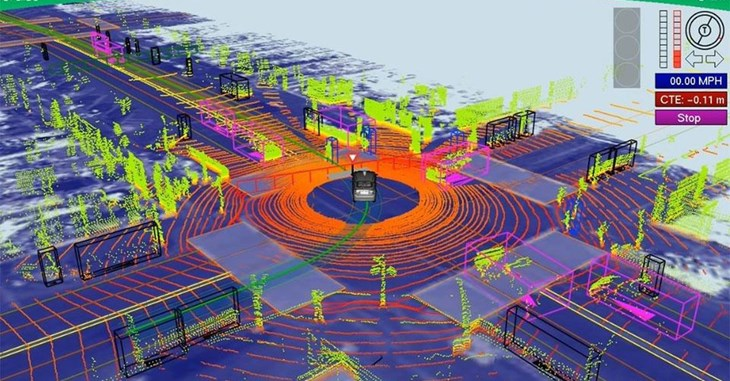
\includegraphics[width=1\linewidth]{Figures/auto-car}
\end{figure*}

\subsection{تعیین موقعیت و تولید تصویر سه بعدی}

پیش از اتخاذ هرگونه تصمیمی برای تعیین مسیر، خودرو باید ابتدا نقشه ای از محیط اطراف خود بسازد و محل خود در این نقشه را با دقت مشخص کند. رایج ترین ابزارهایی که به خودروها در انجام این کار کمک می کنند، دوربین ها و حسگرهای لیزری فاصله یاب هستند. حسگر لیزری با تاباندن پرتوهای لیزر به محیط اطراف و تخمین زمان رفت و برگشت هر پرتو، فاصله خود با اشیاء اطرافش را تعیین می کند. مزیت این روش در مقایسه با استفاده از دوربین ها این است که اطلاعات موردنیاز خودرو سریع تر بدست می آید.

اما این حسگرها خالی از عیب نیز نیستند. برد مفید پرتو لیزر صد متر است و اگر از آن برای ارزیابی فاصله اشیاء در فاصله ای دورتر از صدمتر استفاده شود، کارایی چندانی ندارند. پس از دریافت اطلاعات از هر حسگر، نوبت به فیلترسازی آن می رسد. هدف از این کار، ارسال تنها آن دسته از اطلاعاتی است که برای تعیین مسیر اهمیت دارند و به این ترتیب، از ارسال اطلاعات اضافی به پردازشگر جلوگیری می شود که در نهایت، سرعت عمل و بهره وری پردازشگر را افزایش می دهد. در نهایت، این اطلاعات کنار هم گذاشته می شود تا نقشه ای جامع از محیط پیرامونی شکل بگیرد. حال این نقشه آماده استفاده است تا با کمک آن، بهترین مسیر برای رسیدن خودرو به مقصد نهایی اش تعیین شود.

برای اینکه خودرو بتواند موقیعت اش را به نسبت سایر اشیاء در این نقشه پیدا کند، باید از \lr{GPS}، سیستم ناوبری اینرسی و حسگرهای مختلف استفاده کند. اتکای صرف به \lr{GPS} قابل اطمینان نیست، چرا که احتمال بروز تاخیر در ارسال و دریافت این سیگنال ها بسیار زیاد است. همچنین، برخورد این سیگنال ها با موانع و ساختمان ها نیز موجب کاهش دقت آنها می شود. میزان خطاهای سیستم ناوبری اینرسی نیز در طول زمان زیاد است و به همین دلیل، الگوریتم های مسیریابی اطلاعات موردنیاز خود برای تصمیم گیری را از منابع مختلفی دریافت می کنند. طی هر لحظه ای که خودرو حرکت می کند، اطلاعات جدیدی تولید می شود و در نتیجه، نقشه بروزرسانی می شود.

\subsection{اجتناب از موانع}

نقشه درونی هر خودرو شامل موقعیت کنونی تمام موانع ثابت (مانند ساختمان ها، چراغ های راهنمایی و رانندگی، نشانه های توقف) و متحرک (سایر خودروها و عابرین پیاده) اطراف آن می شود. تعیین نوع مانع، ثابت یا متحرک، توسط الگوریتمی تعیین می شود که سعی می کنند تصویر هر مانع را با مجموعه ای از تصاویری که از قبل در آن بارگذاری شده مقایسه کرده و نزدیک ترین شکل به آن را تشخیص دهد. برای مثال، اگر وسیله نقلیه ای با دو چرخ و با سرعت هشتاد کیلومتر در حال حرکت در نزدیکی خودرو باشد، به احتمال زیاد موتور سیکلت است و دوچرخه نیست، و بر همین اساس توسط الگوریتم خودرو دسته بندی می شود.

همچنین، این الگوریتم تلاش می کند تا با اتکا به یک الگوریتم احتمال گرا، مسیر احتمالی اشیاء متحرک را پیش بینی کند. به این ترتیب، خودرو امکان اتخاذ تصمیمات هوشمندانه تری را به هنگام نزدیکی به مناطق پرتردد را پیدا می کند. تمام موقعیت ها و مسیرهای احتمالی پیش بینی شده در اختیار مرکز پردازش قرار می گیرند تا در بروزرسانی های لحظه ای نقشه، اعمال شوند.

\subsection{تعیین مسیر}

هدف از فرایند تعیین مسیر، استفاده از اطلاعات بدست آمده از نقشه خودرو به منظور رسیدن به مقصد با سلامت کامل و بدون مواجهه با موانع جاده و همچنین پیروی از قوانین راهنمایی و رانندگی است. اگرچه ممکن است راه و روشی که هر خودروساز برای اتومبیل خودران خود انتخاب می کند کم و بیش متفاوت باشد، اما منطق بکار رفته در همه آنها یکسان است و در ادامه به شرح آن می پردازیم.

در ابتدا یک راه اصلی و کامل برای خودرو تعیین می شود تا با دنبال کردن آن به مقصد برسد. در عین حال، هر لحظه تغییراتی در مسیرهای مقطعی ایجاد می شود تا عیوب آن برطرف شده و بهترین مسیر بدست آید. این الگوریتم همچنین تلاش می کند تا بهترین مسیر را براساس حرکت خودروهای اطراف پیدا کند. فرض کنید خودرویی در فاصله پنج متری خودروی شما در حال حرکت است و شما قصد دارید تا در اولین خروجی به سمت راست بپیچید. در چنین شرایطی اگر با همین سرعت ادامه مسیر دهید قطعا امکان دسترسی به خروجی را نخواهید داشت چرا که مسیر شما مسدود است. پس خودرو تصمیم می گیرد تا از سرعت خود کم کند تا خروجی را از دست ندهد. به همین منظور، دستوراتی به تمام عملگرهای مکانیکی داده می شود تا سرعت خودرو کم شده و پس از عبور خودروی جانبی، راه برای رسیدن به خروجی باز شود. جالب است بدانید که تمام این محاسبات طی زمانی کمتر از 50 میلی ثانیه انجام می شود. البته این مدت زمانی به طور متوسط است و ممکن است بنابر شرایط مختلف، این زمان کوتاه تر یا بلندتر نیز بشود. قدرت پردازشگر، حجم اطلاعات دریافت شده و پیچیدگی مسیر پیش رو نیز بر مدت زمان تصمیم گیری خودرو تاثیر می گذارد.

تمام این فرایندها آنقدر ادامه پیدا می کنند تا خودرو به مقصد برسد و مسافران به سلامت از آن پیاده شوند.

خودروسازان طی یک دهه اخیر در زمینه تحقق بخشیدن به رویای خودروهای خودران دستاوردهای زیادی داشته اند. با این حال، هنوز هم موانع فنی زیادی در این راه وجود دارد که باید پیش از ورود خودروهای خودران به بازار برطرف شوند. سیگنال های \lr{GPS} هنوز به طور کامل قابل اطمینان نیستند، سیستم های بصری کامپیوتری با مشکلاتی در شناسایی علائم جاده ای روبرو هستند و شرایط آب و هوایی نیز تا حد زیادی روی عملکرد پردازشگرهای خودروها و تشخیص و تصمیم گیری صحیح آنها اثرگذاراند.

با این حال، این موانع قابل حل شدن هستند. هر روز خبرهای تازه ای از طراحی و تولید پردازنده های قدرتمندتر و الگوریتم های بهینه تر به گوشی می رسد و به همین نسبت، از میزان تصادفات خودروهای خودران کاسته می شود. امروزه خودروهایی هستند که به طور نمیه خودران حرکت می کنند و راننده از انجام بسیاری ازکارها، از جمله پارک کردن خودرو معاف کرده اند. پس باید منتظر بود و دید که طی چند سال آینده، چه دستاوردهایی در صنعت خودروسازی حاصل می شود و کدام یک از شرکت های خودروساز موفق می شود تا نام خود را به عنوان نخستین عرضه کننده خودروی خودران در تاریخ ثبت کند.


\section{بررسی مقدماتی \ws{rl}}

\subsection{جایگاه \ws{rl} در \ws{ml}}
بسیاری از صاحب نظران \w{ml} را به سه دسته تقسیم می‌کنند :
\begin{enuminline}
	\item \w{supLearning}
	\item \w{unsupLearning} یا \w{clustering}
	\item \w{semisupLearning}
\end{enuminline}

در این میان،
\w{rl}
را بعضی ها دسته چهارم می‌دانند و  بعضی دیگر آن‌را در دسته سوم قرار می‌دهند. بر اساس دسته‌بندی گروه دوم شکل 
\ref{fig:rl-machinelearning-chart}
رسم شده است.


همچنین شکل 
\ref{fig:rl-chart}
کابرد \w{rl} را در علوم مختلف نشان می‌دهد.

\begin{figure}[h!]
	\centering
	\def\localheigth{7cm}
	\subfigure[]{%
		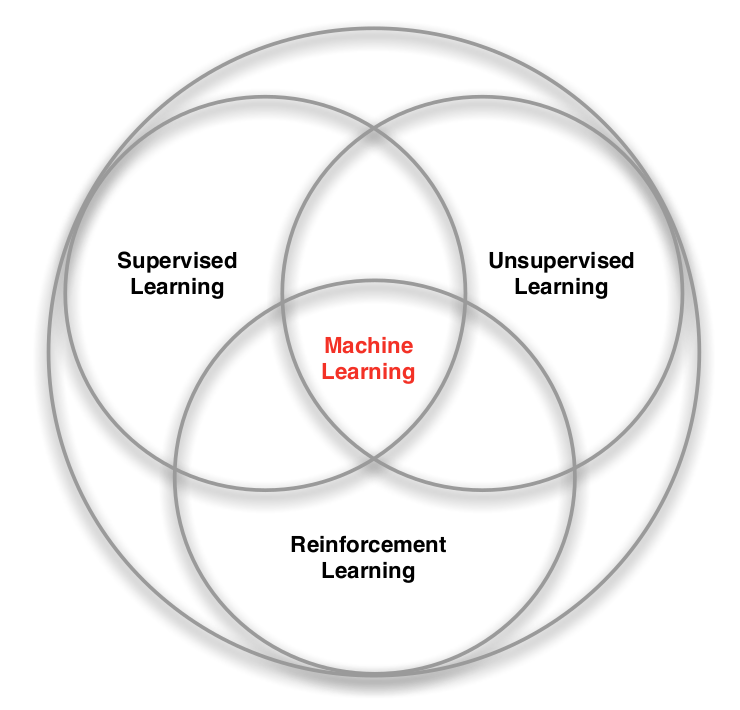
\includegraphics[height=\localheigth]{Figures/RL/RL-machinelearning-chart}
		\label{fig:rl-machinelearning-chart}
	}
	%  	\hspace*{1.5cm} % space between two figures
	\subfigure[جایگاه \lr{RL} در علوم مختلف]{%
		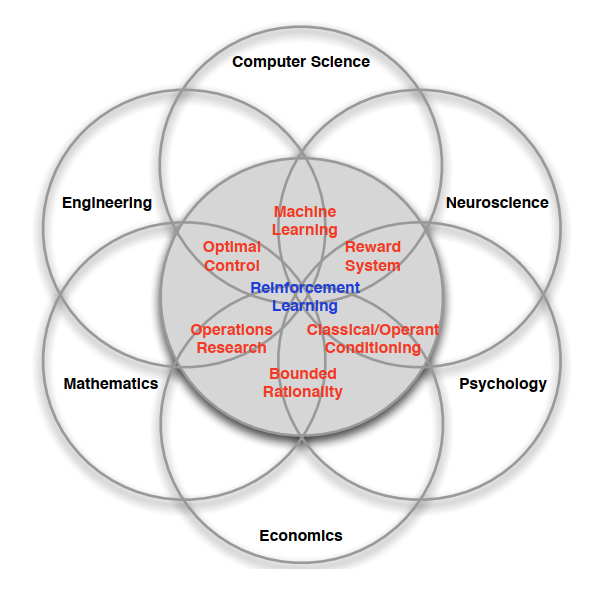
\includegraphics[height=\localheigth]{Figures/RL/RL-chart}
		\label{fig:rl-chart}
	}
	\caption{%
		جایگاه \ws{rl}
	}
	\label{fig:Rl-circle-total}
\end{figure}



\subsection[وجه تمایز 
\ws{rl}
از دیگر الگو‌های 
\ws{ml}
]{چه چیزی 
\ws{rl}
را با دیگر الگوهای 
\ws{ml}
متمایز می‌کند؟
}

این سوال از آن جهت حایز اهمیت است که بیان می‌کند چرا ما به سراغ الگوی 
\w{rl}
رفته‌ایم. پاسخ ملاحظات زیر است.

\begin{alphabetlist}
\item هیچ 
\w{sup}
وجود ندارد و صرفا \w{reward}ها وجود دارند.
\item 
\w{feedback}
همراه با تاخیر است وبه صورت همزمان رخ نمی‌دهد.
\RTLfootnote{در مورد علت تاخیر در ادامه توضیح داده خواهد شد.}
\item 
مفهوم زمان واقعا مطرح است و یک ترتیب خاص از داده ها داریم.
شکل \ref{fig:markov-chain-sarsa} این توالی زمانی را نشان می‌دهد.
\end{alphabetlist}

\w{rl}(\gls{a:rl})
بر اساس \w{rewardhypo} پایه‌گذاری می‌شود.
\begin{definition}[\w{rewardhypo}]
	همه اهداف می‌توانند براساس بیشینه کردن مقدار میانگین تجمعی امتیازها توصیف کرد.
\end{definition}

ممکن است این عبارت کمی عجیب بنظر برسد اما در بسیاری از مسایل که به صورت برد و باخت و به نوعی دو حالت مطلوب و نامطلوب دارند، می‌توان در ساده ترین حالت مقدار $+1$ را برای برد و $-1$ را برای باخت در نظر گرفت.

\begin{remark}
	در برخی منابع بجای \w{reward} از مفهوم \w{cost} استفاده می‌کنند و هدف الگوریتم آن می‌شود که به سمتی حرکت کند که کمترین \w{cost} را داشته باشد. برای یک‌پارچه‌سازی این مفاهیم معمولا یک علامت منفی برای این دو در نظر میگیرند یعنی :
	\[	\text{\rl{\w{reward}}} = -\text{\rl{\w{cost}}}
		\quad \colon \quad
		r = -c
		\]
\end{remark}

\subsection{
\ws{agent} و \ws{env}
}
 
 این مفهوم بسیار مفهوم مهمی می‌باشد و بارها از آن در این پروژه یاد شده است.
 
 در مسایل \w{rl} یک 
 \textbf{\w{agent}}
 وحود دارد که در یک \textbf{\w{env}} درحال تعامل است. \w{env} می‌تواند محیط اطراف \w{agent} باشد و یا هرچیزی که \w{agent} با آن در تعامل است.
  \cite{uclRL}
\begin{figure}[t]
	\centering
	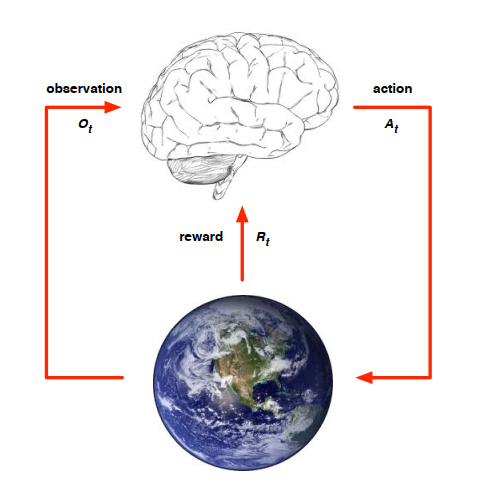
\includegraphics[width=0.7\linewidth]{Figures/RL/Enviroment-brain-as-agent}
	\caption{تعامل \w{agent} و \w{env}}
	\label{fig:enviroment-brain-as-agent}
\end{figure}

این تعامل به این صورت است که \w{agent} که در ابتدا یک \w{state} اولیه دارد، یک \w{action} بر روی \w{env} در زمان $t$ انجام می‌دهد. 
\w{env} مقدار \w{action} در زمان $t$ را دریافت می‌کند و 
سپس \w{env} در زمان $t+1$ دو اطلاعات مهم را بر می‌گرداند. 
\begin{alphinline}
	\item \w{obs}
	\item \w{reward}
\end{alphinline}

شکل 
\ref{fig:enviroment-brain-as-agent}
و \ref{fig:markov-chain-sarsa}
این تعامل را نشان می‌دهد. لازم به ذکر است که در پایان هر \w{step} مقدار $t$ یک واحد افزایش می‌یابد.

\subsection{\ws{state}}
در بخش قبل تعریف مناسبی از \w{state} ارایه نشد. برای این تعریف ابتدا مفهوم \w{history} ارایه می‌شود و از روی آن \w{state} تعریف خواهد شد.

\begin{definition}[\w{history}]
	به سری شامل \w{obs}، \w{action} و \w{reward} می‌باشد:
	\[
	\mathcal{H}_t = \mathcal{O}_1 ,\mathcal{R}_1, \mathcal{A}_1, \dots, \mathcal{A}_{t-1}, \mathcal{O}_{t-1}, \mathcal{R}_t
	\]
\end{definition}


\begin{figure}[t]
	\centering
	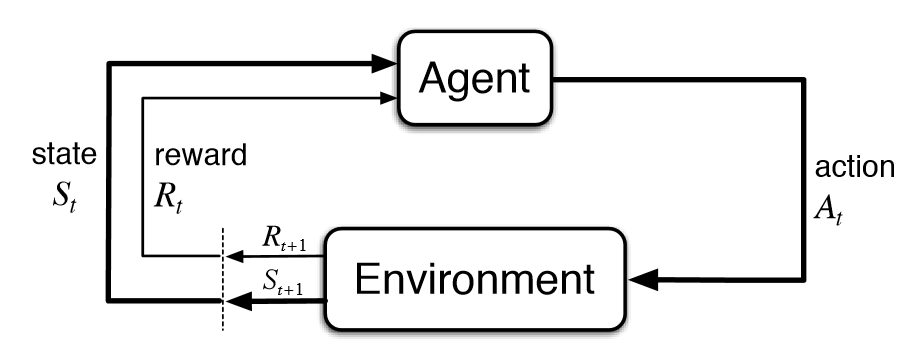
\includegraphics[width=0.7\linewidth]{Figures/RL/Markov-vhain-SARSA}
	\caption{شماتیک تعامل محیط با عامل}
	\label{fig:markov-chain-sarsa}
\end{figure}

با این تعریف \w{state} را می‌توان به شکل زیر تعریف کرد.

\begin{definition}\label{def:state}
	\textbf{\w{state}}
	اطلاعاتی است که در محاسبات برای آن‌که در بعد چه اتفاقی بیافتد، استفاده می‌شود. به عبارت دیگر \w{state} تابعی از \w{history} می‌باشد.
	\[
	\mathcal{S}_t = f(\mathcal{H}_t)
	\]
\end{definition}

دو نوع \w{state} وجود دارد.
\begin{alphabetlist}
	\item \textbf{\w{env state}} که با علامت $S_t^e$ نشان داده می‌شود.
	اطلاعات نهان \w{env} را نشان می‌دهد و معمولا برای \w{agent} به‌طور کامل دیده نمی‌شود. حتی اگر برای \w{agent} مشاهده‌پذیر نیز باشد، ممکن است اطلاعات کاملا بی‌ربطی را همراه داشته باشد.
	\item \textbf{\w{agent state}} که با علامت $S_t^a$ نشان داده می‌شود.
	که برابر است با هر اطلاعاتی که \w{agent} برای رسیدن به \w{action} بعدی با استفاده از الگوریتم های \gls{a:rl} استفاده می‌کند. 
\end{alphabetlist}

بنابراین در نعریف \ref{def:state} مناسب‌تر است بجای واژه \w{state} از \w{agent state} استفاده شود. بنابراین:
	\[
	\mathcal{S}_t^a = f(\mathcal{H}_t)
	\]
	
\begin{note}
	از این پس در سراسر این پایان‌نامه هرجا صحبت از \w{state} شد منظور همان \w{agent state} است.
\end{note}
	
\begin{definition}
	یک 
	\w{state}
	$\mathcal{S}_t$
	\w{markov}
	است اگر و تنها اگر:
	$$
		\mathbb{P}\left[\mathcal{S}_{t+1} | \mathcal{S}_{t}\right]=\mathbb{P}\left[\mathcal{S}_{t+1} | \mathcal{S}_{1}, \ldots, \mathcal{S}_{t}\right]
	$$
\end{definition}
در یک \w{markov state}، آینده از گذشته مستقل است و فقط به زمان حال وابسته است.
و این به این معناست که \w{state} از لحاظ آماری برای توصیف آینده کافی است.

\begin{remark}
	\w{env state} $S_t^e$  \w{markov} است.
	همچنین 
	\w{history} نیز \w{markov} است.
\end{remark}


\subsection{\ws{observ}}

\subsubsection{\ws{fullobs}}

\w{agent}
به‌طور مستقیم \w{env state} را مشاهده می‌کند. بنابراین در این حالت داریم:
	\[
		\mathcal{O}_t = \mathcal{S}_t^a = \mathcal{S}_t^e
	\]
بنابراین در این حالت عبارت های زیر با یک‌دیگر برابر هستند.
	\[
	\text{\rl{\w{agent state}}} = \text{\rl{\w{env state}}} = \text{\rl{\ws{info state}}}
	\]\RTLfootnote{\w{info state}
	مفهومی مانند \w{markov state} دارد.
}
به صورت رسمی، این فرایند یک \Glspl{w:mdp}(\gls*{a:mdp}) می‌باشد.
\cite{Sutton1998}
	

\subsubsection{\ws{partialobs}}
\w{agent} به‌طور غیر مستقیم \w{env} را مشاهده می‌کند.
\begin{example}
			یک ربات با دید دوربین نمی‌تواند موقعیت مطلق را اعلام کند.		
\end{example}
\begin{example}
	یک اتومبیل با سنسور تشخیص فاصله نمی‌تواند اطلاعاتی مانند نوع ماشین و قیمت آن را تشخیص دهد.
\end{example}

\subsection{\ws{pol}}
\w{pol}
در حقیقت تابعی احتمالی و یا معین است که تصمیم می‌گیرد که در \w{state} کنونی چه تصمیمی باید گرفت. در واقع رفتار \w{agent} توسط این تابع، بررسی و نشان داده می‌شود.

\begin{definition}
	اگر تابع معین باشد این تابع به صورت زیر تعریف می‌شود.
$$
a = \pi(s)
$$
و اگر تابع احتمالاتی باشد به صورا زیر تعریف می‌شود.
$$
\pi(a | s)=\mathbb{P}\left[A_{t}=a | S_{t}=s\right]
$$
\end{definition}


\section{مطالعه بیشتر}
جهت مطالعه بیشتر و آشنایی با ادبیات یادگیری تقویتی و همچنین الگوریتم های آن می‌توانید به مرجع  \cite{Sutton1998} و \cite{uclRL}
مراجعه کنید.



%$$
%\tilde{v}_{\pi}(s)=\mathbb{E}_{\pi}\left[\sum_{k=1}^{\infty}\left(R_{t+k}-\rho^{\pi}\right) | S_{t}=s\right]
%$$





%\begin{figure}
%	\centering
%	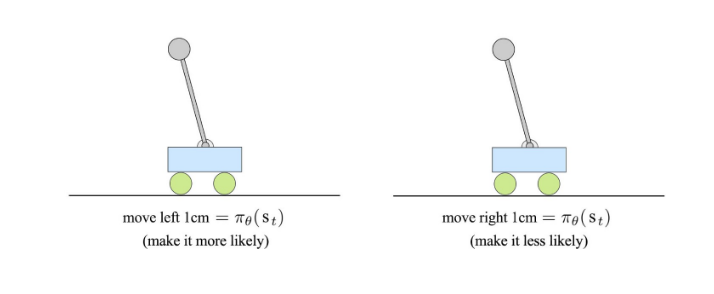
\includegraphics[width=0.7\linewidth]{Figures/RL/RL-cartpole}
%	\caption{}
%	\label{fig:rl-cartpole}
%\end{figure}





\section{پیشنیاز های نصب و معرفی قسمت های مختلف}\label{ch:req}

\subsection{نرم‌افزار‌های کلی}
در این پروژه از جهت آنکه نسخه قبلی و پیشینی برای  آن نبوده است، به ناچار می‌بایست که کد آن از صفر تا صد آن به صورت دستی نوشته شود. از این‌رو، پیچیدگی های بسیار فراوان را به طور خاص در پی داشت. ابزار های زیادی نیز بنابه شرایط در آن استفاده شد که ارتباط بین آن ابزار ها و اجزا، بر این پیچیدگی پیاده سازی طرح افزوده بود.

ابزار های اصلی و کلی که در این پروژه استفاده شده بود، عبارتند از:

\begin{itemize}
	\item 
	\textbf{نرم افزار 
		\glspl{w:prescan}}
	، نسخه \lr{$8.5.0$}
	
	\item 
	\textbf{نرم افزار 
		\glspl{w:matlab}	
	}
	، نسخه \lr{R2017b}
	\item 
	\textbf{زبان برنامه نویسی پایتون}
	، نسخه \lr{$3.6.9$}
\end{itemize}

بنابراین برای راه اندازی مجدد کد این پروژه لازم است که موارد بالا روی کامپیوتر شخص به صورت کامل نصب باشد.

همچنین لازم به ذکر است که برخی ابزارات دیگر نیز در این پروژه استفاده شده است که احتمالا با نصب موارد بالا دیگر نیازی به نصب آن ها به صورت جداگانه نیست. هدف این ابزار ها ایجاد اتصال بین اجزای اصلی گفته شده است. این گروه شامل موارد زیر هستند:

\begin{itemize}
	\item 
	\textbf{\glspl{w:simulink}}
	، جهت اتصال بین متلب و پری اسکن
	
	\item 
	\textbf{شبکه \lr{UDP}}
	\RTLfootnote{برای این منظور از ماژول \lr{socket} در پایتون استفاده شده است. }
	، جهت اتصال داده های پویا 
	\LTRfootnote{Dynamic Data}
	بین پایتون و سیمولینک
	
	\item \textbf{\glspl{w:matlabengine}}
	، جهت اتصال داده های ساکن
	\LTRfootnote{Static Data}
	بین پایتون و سیمولینک
\end{itemize}

در این فصل جزئیات بیشتری در مورد لزوم و دلیل استفاده از این ابزار ها بررسی می‌شود.




\subsection{پیشنیاز های پایتون}

\begin{note}
	
	کد پایتون در این پروژه شامل دو قسمت کلی زیر می‌شود. این دو دسته در شکل
	\ref{fig:python-layers-env-alg}
	مشخص هستند.
	\begin{enumerate}
		\item 
		دسته اول مربوط به آن بخش از پروژه است که وظیفه اصلی آن ارتباط پیدا کردن با محیط متلب و پری اسکن و ایجاد یک نوع واسط کاربری است. گرفتن و فرستادن اطلاعات مخصوص این قسمت است.
		\item 
		دسته دوم با محیط و نحوه ارتباط آن کاری ندارد و تمرکز خود را بر‌روی الگوریتم خود که در این جا از الگوریتم های یادگیری تقویتی استفاده شده است، قرار داده است.
	\end{enumerate}
	
\end{note}

\begin{figure}
	\centering
	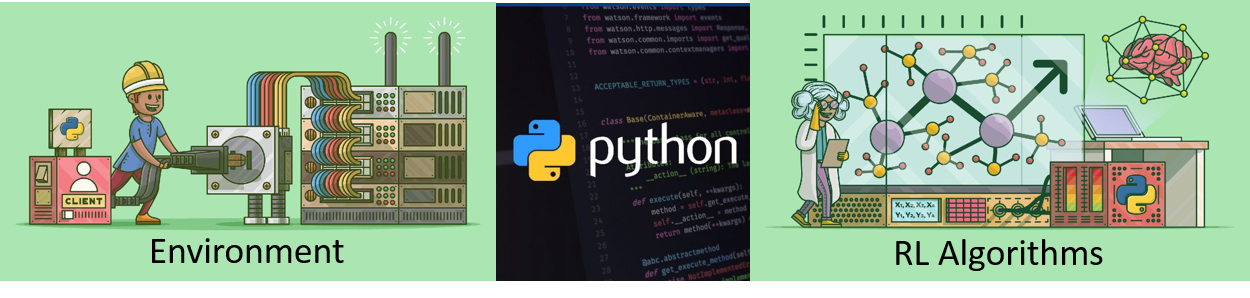
\includegraphics[width=\linewidth]{Figures/python-layers-env-alg}
	\caption{تقسیم بندی وظایف اصلی کد پایتون}
	\label{fig:python-layers-env-alg}
\end{figure}


دسته اول (سمت چپ تصویر
\ref{fig:python-layers-env-alg}
)
به پکیج های زیر احتیاج دارد:
\begin{multicols}{3}
	\begin{itemize}
		\item \lr{numpy} \item \lr{socket} \item\lr{time} و \lr{os} \item \lr{pandas}
		\item \lr{matlab.engine} \item \lr{gym}
	\end{itemize}
\end{multicols}
اگر از 
\glspl{w:anaconda}
برای پایتون استفاده می‌کنید غیراز دو بسته 
\lr{gym}
و 
\lr{matlab.engine}
به صورت پیش‌فرض نصب شده اند در صورت عدم نصب آن ها را با استفاده از 
\lr{pip}\RTLfootnote{مثلا بسته \lr{numpy} را با استفاده از دستور \lr{\texttt{pip install numpy}} نصب می‌توان کرد.}
می‌توان نصب کرد.

بسته \lr{gym} که در این فصل به‌تفصیل در مورد آن بحث شده است، به راحتی با همان دستور \texttt{pip} نصب می‌شود. اما نصب 
\lr{matlab.engine}
یا همان
\glspl{w:matlabengine}
متفاوت است و نمی‌توان آن را نیز به همان روش نصب کرد.

دسته دوم شامل بسته های زیر است:
\begin{itemize}
	\item \lr{gym[atari]} یا \lr{gym[all]}
	\item \lr{tensorflow}
	\item \lr{stable-baseline}
	
\end{itemize}

این بسته ها در لایه الگوریتم استفاده شده است.(در مورد این لایه در فصل 
\ref{ch:alg}
بیشتر صحبت خواهد شد.)
هر سه‌تای این بسته ها با همان دستور \lr{pip} به راحتی نصب می‌شوند.



\subsection{معرفی دقیق تر اجزای کلی}
در این قسمت میخواهیم سه نرم‌افزار کلی این پروژه را از نگاهی نزدیک تر  بشناسیم که عبارتند از :
\begin{enuminline}
	\item 
	نرم‌افزار 
	\glspl{w:prescan}
	\item 
	\glspl{w:matlab}
	\item پایتون
\end{enuminline}

\subsection{معرفی نرم‌افزار 
	\ws{prescan}
}

پس از دانلود و نصب نسخه \lr{8.5.0} این نرم‌افزار چهار آیکون مانند شکل 
\ref{fig:prescan-icons}
به محیط دسکتاپ اضافه می‌کند.  اصلی ترین آن ها 
\lr{PreScan Proccess Manager 8.5.0}
نام دارد.

\begin{figure}[h]
	\centering
	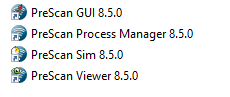
\includegraphics[width=0.4\linewidth]{Figures/prescan-icons}
	\caption{آیکون های اضافه شده بر روی محیط دسکتاپ پس از نصب پری‌اسکن}
	\label{fig:prescan-icons}
\end{figure}

با انتخاب آن صفحه ای مانند زیر باز می‌شود.

\begin{figure}[h]
	\centering
	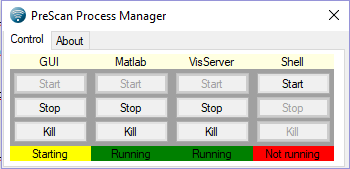
\includegraphics[width=0.5\linewidth]{Figures/Prescan-panel}
	\caption{پنل مدریت نرم‌افزار پری‌اسکن}
	\label{fig:prescan-panel}
\end{figure}

این پنجره شامل گزینه های زیر است:
\begin{multicols}{2}
	\begin{itemize}
		\item \lr{GUI}
		\item \lr{VisServer}
		\item \lr{Matlab}
		\item \lr{Shell}
	\end{itemize}
\end{multicols}

برای ایجاد یک محیط جدید باید \lr{GUI} را استارت کرد. پس از مدتی صفحه ای مانند شکل 
\ref{fig:prescan-gui}
باز می‌شود. 


\begin{figure}
	\centering
	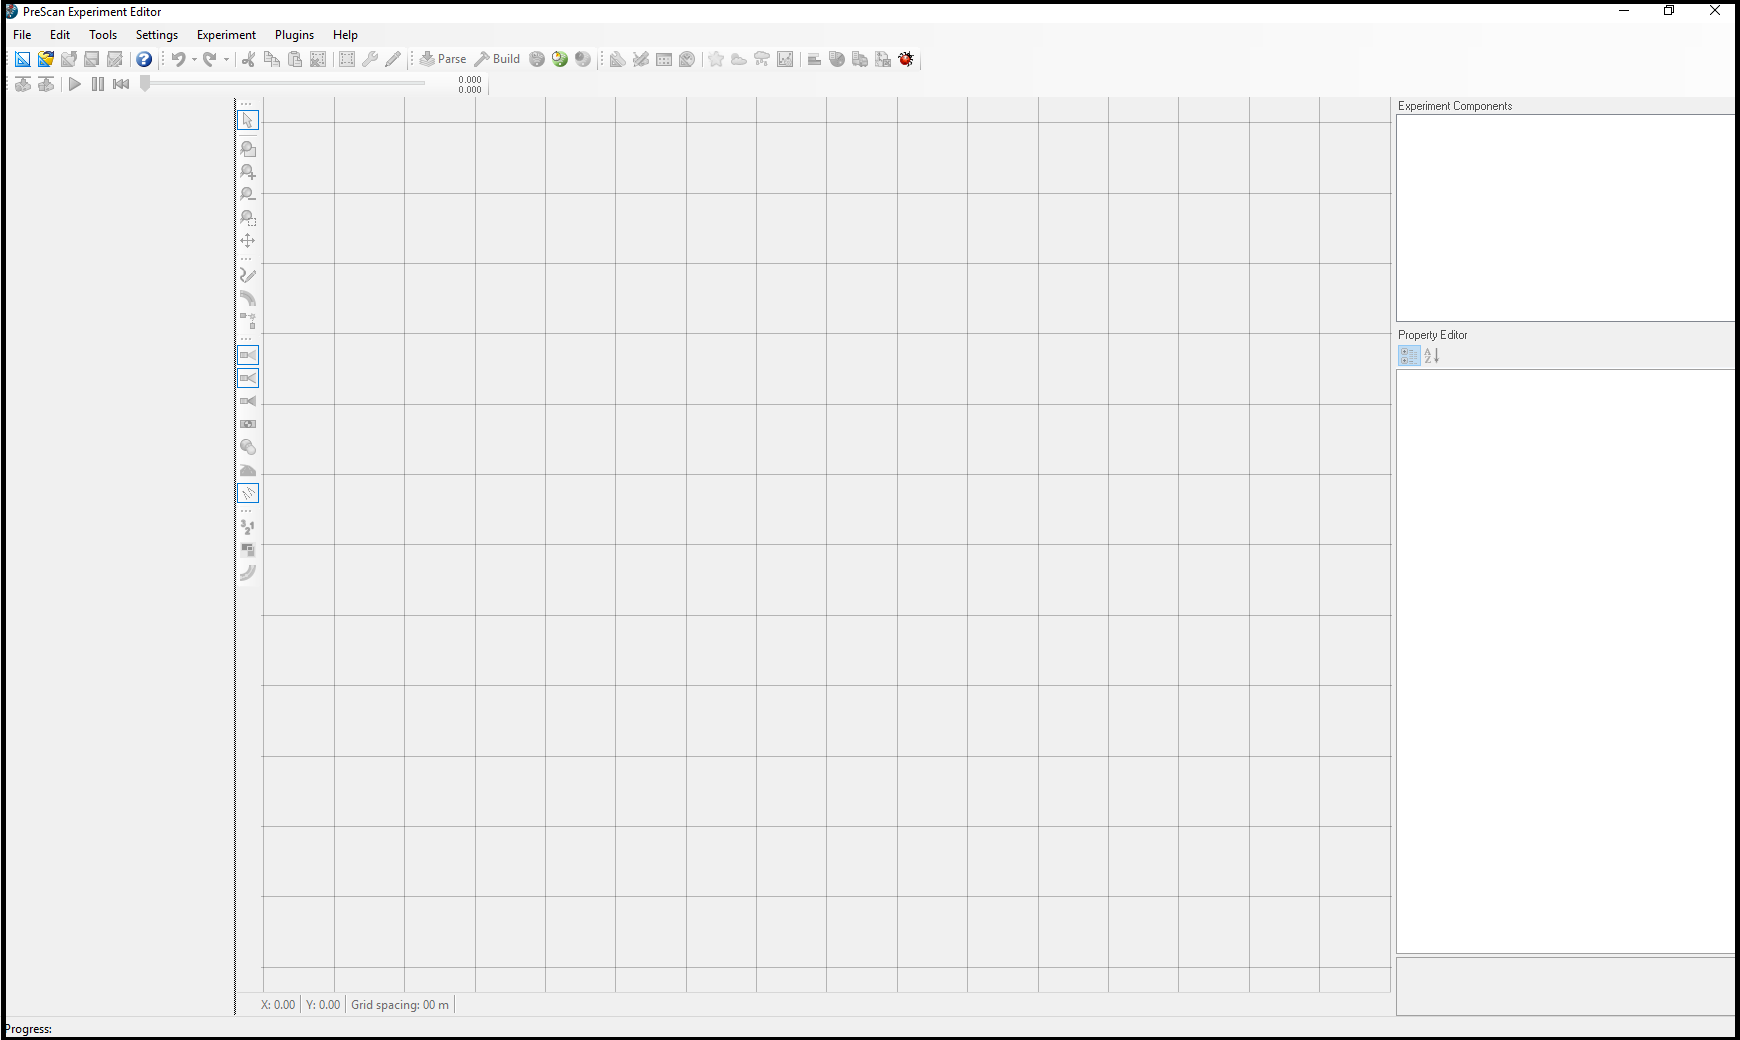
\includegraphics[width=0.7\linewidth]{Figures/Prescan-GUI}
	\caption{صفحه گرافیکی محیط پری‌اسکن}
	\label{fig:prescan-gui}
\end{figure}

پس از ایجاد مدل ها و ذخیره آن، فایل های \texttt{**.pex} و \texttt{**.pb} و \texttt{**\_cs.slx} ساخته می‌شود.
\RTLfootnote{علامت ** به معنای یک اسم مشترک در این سه فایل استفاده شده است. }

جهت استفاده از فایل سیمولینک باید در شکل 
\ref{fig:prescan-panel}
متلب را استارت کنید.
\begin{remark}
	برای اجرای فایل های سیمولینک خروجی، لازم است که متلب را فقط و فقط با استفاده از نرم افزار پری‌اسکن و با استفاده از پنل مدیریت نرم افزار معرفی شده در شکل 
	\ref{fig:prescan-panel}
	باز شود. در صورتی که به صورت مستقیم این کار انجام شود، به مشکل منتهی می‌شود.
\end{remark}


دو قسمت دیگر نیز در شکل 
\ref{fig:prescan-panel}
وجود دارد که نیازی به استارت کردن آن ها نیست و خودشان در صورت لزوم به صورت خودکار فراخوانی می‌شوند.

\subsection{فرمت های فایل های خروجی}
نرم‌افزار پری‌اسکن پس از ایجاد یک محیط جدید، فایل ها و پوشه های بسیار زیادی را ایجاد می‌کند. اما در خارج آن پوشه ها ۳ فایل وجود دارد که پسوند آن ها \texttt{**.pex} و \texttt{**.pb} و \texttt{**\_cs.slx} می‌باشد. علامت ** همان اسم پروژه‌ای است که ایجاد کرده ایم. هر یک از این فایل ها به یک بلوک از شکل 
\ref{fig:block-diagram}
مربوط می‌شود.

\begin{table}[h!]
	\tableset{
		%{\setcellgapes{0.5em}\makegapedcells
		\begin{tabular}{|C{0.15\linewidth}|p{0.8\linewidth}|}
			\hline\rowcolor{lightgray}
			فرمت فایل
			&
			توضیحات 
			\\\hline\hline
			\texttt{**.pex} &	این فایل مربوط به اولین بلوک شکل
			\ref{fig:block-diagram}
			است و ارتباط مستقیم با \lr{GUI} دارد. برای تغییر محیط گرافیکی باید این فایل را باز کرد.
			\\ \hline   
			\texttt{**.pb} & این فایل برخی از اطلاعات فایل 
			\texttt{**.pex}
			را در اختیار دارد و با تغییر آن فایل این فایل نیز عوض می‌شود. این فایل حاوی اطلاعات استاتیک محیط ایجاد شده است و مهم ترین کاربرد آن در بلوک موتور متلب که در شکل 
			\ref{fig:block-diagram}
			نشان داده شده است می‌باشد. پایتون از طریق این فایل این اطلاعات را دریافت می‌کند.
			\\\hline
			\texttt{**\_cs.slx} &
			این فایل سیمولینک است که برای کار کردن با آن باید از پنل مدیریت شکل
			\ref{fig:prescan-panel}
			استفاده کرد. این فایل پس از ایجاد از فایل 
			\texttt{**.pex}
			مستقل می‌شود. این فایل خود قابلیت تغییر دارد و می‌توان بلوک‌های آن‌را در محیط سیمولینک تغییر داد و بلوک های دیگری به آن افزود.  در صورتی که فایل \texttt{**.pex} تغییر کند، این امکان را نیز دارد که از داخل خود سیمولینک با فشردن دکمه ای این تغییرات جدید اعمال شود بدون آن که به تغییرات خود کاربر لطمه ای وارد شود. در این پروژه این فایل، تغییرات بسیاری را تجربه کرد.
			\\\hline
	\end{tabular}}
	\caption{توضیحات فرمت فایل خروجی}
	\label{tab:prescan-format}
\end{table}



جدول
\ref{tab:prescan-format}
توضیحات لازم را جهت آشنایی با این خروجی ها آورده است.

همچنین در بخش  
\ref{ch:fani|sec:simulink}
در مورد فایل \texttt{**\_cs.slx} توضیحات دقیق‌تری در مورد جزییات آن گفته خواهد شد.





\subsection{نصب
	\ws{matlabengine}
}
برای نصب موتور متلب ابتدا نیاز است که به متلب به طور کامل در سیستم نصب باشد. پس از نصب متلب، محیط \lr{Command prompt (admin)} را باز کنید و با توجه به نسخه و محل نصب متلب خود به آدرس زیر بروید.

\begin{center}
	\LRE{\verb|<matlabroot>\extern\engines\python|}
\end{center}

مثلا برای \lr{Matlab R2017b} که در محل پیش‌فرض خود نصب شده باشد این کار با استفاده از دستور زیر انجام می‌شود.

\begin{center}
	\LRE{\verb|cd C:\Program Files\MATLAB\R2017a\extern\engines\python|}
\end{center}

در این پوشه یک فایل به نام \lr{setup.py} موجود می‌باشد. این فایل را با استفاده از دستور 

\begin{center}
	\LRE{\verb|python setup.py install|}
\end{center}

در همان محیط \lr{cmd} اجرا کنید.

\begin{note}
	توجه داشته باشید که باید نسخه متلب و پایتون شما باید با یکدیگر سازگار باشند. برای بررسی این موضوع اگر فایل \lr{setup.py} را با اسنفاده از یک ادیتور باز کنید، یک آرایه به نام \texttt{\_supported\_versions} در آن خواهید دید. مقادیر این آرایه، نسخه هایی از پایتون را نشان می‌دهد که توصط نسخه متل شما پشتیبانی میشود مثلا در این مورد، با توجه به خط زیر نسخه های $2.7$ ، $3.4$ ، $3.5$ و $3.6$ پاینون پشتیبانی می‌شود. در غیر این صورت باید نسخه سازگار متلب و یا پایتون را نصب کنید.
	\begin{center}
		\lr{\texttt{\_supported\_versions = ['2.7', '3.4', '3.5', '3.6']}}
	\end{center}
\end{note}

\section{معرفی دقیق تر پیشنیاز های پایتون}\label{ch:req|sec:python-req}
\subsection{بسته‌های کمکی}
این بسته ها نقش حیاتی ندارند و برای برخی از موارد استفاده شده‌اند. این موارد در جدول
\ref{table:aux-packages}
آمده است.

\begin{table}[t!]\tableset{
		\begin{tabular}{|C{0.13\linewidth}|C{0.52\linewidth}|C{0.25\linewidth}|}
			\hline\rowcolor{lightgray} نام بسته  &  دلیل استفاده & روش نصب
			\\\hline\hline
			\lr{numpy} & ایجاد ماتریس برای \glspl{w:actionspace} و \glspl{w:obsspace} & \LRE{\texttt{pip install numpy}}
			\\\hline
			\lr{time} & جهت ایجاد تاخیر و 
			\glspl{w:timeout}
			& \LRE{\texttt{pip install time}}
			\\\hline
			\lr{os} & برای بستن پنجره های باز شده پس از اجرا & \LRE{\texttt{pip install os}}
			\\\hline
			\lr{pandas} & برای چاپ اطلاعات آماری 
			\glspl{w:reward}
			های بدست آمده در پایان هر 
			\glspl{w:episode}
			& \LRE{\texttt{pip install pandas}}
			\\\hline
			\lr{socket} & برقراری ارتباط با 
			\w{matlab}
			و فرستان و دریافت کردن 
			\ws{dyndata}
			& \LRE{\texttt{pip install socket}}
			\\\hline
			\lr{tensorflow} & برای لایه الگوریتم و استفاده از الگوریتم‌های
			\w{drl}
			& \LRE{\texttt{pip install tensorflow}}
			\\\hline
	\end{tabular}}
	\caption{معرفی بسته های کمکی پایتون و علت استفاده از آن‌ها}
	\label{table:aux-packages}
\end{table}

\subsection{بسته \lr{gym}}

\subsubsection{معرفی}
بسته 
\href{https://github.com/openai/gym}{\lr{gym}}
که توسط 
\href{https://github.com/openai}{\lr{OpenAI}}
توسعه یافته است. این ابزار فوق العاده این امکان را برای محقیقین علوم کامپیوتر حرفه‌ای و یا آماتور فراهم می‌کند که انواع الگوریتم های 
\w{rl}
(\gls*{a:rl})
را بر روی کار خود تست کنند. همچنین پتانسیل این را دارد که محقیقن محیط خود را برروی این بسته توسعه دهند.

هدف از ایجاد این بسته، استاندارد سازی 
\w{env}
و نوعی 
\w{benchmark}
برای پژوهش های 
\gls*{a:rl}
محسوب می‌شود.\cite{medgyminstall}

در حقیقت می‌توان این بسته را در وسط شکل
\ref{fig:python-layers-env-alg}
جای‌ داد. جایی که لایه 
\w{env}
و لایه 
\w{alg}
به‌یک‌دیگر می‌رسند. 

این بسته محیط هایی از پیش ساخته شده دارد. نام این بسته ها در لیست زیر
آمده است. 
\RTLfootnote{جدول کامل در سایت 
	\url{https://github.com/openai/gym/wiki/Table-of-environments}
	قرار دارد. 
}
اکثر این محیط ها نوعی بازی هستند که 
\w{agent}
سعی در یادگیری آن محیط ها دارد.


\begin{multicols}{2}\scriptsize\setstretch{0.5}
	\begin{itemize}
		\item \lr{CartPole-v0}
		\item \lr{Pendulum-v0}
		\item \lr{MountainCar-v0}
		\item \lr{MountainCarContinuous-v0}
		\item \lr{BipedalWalker-v2}
		\item \lr{Humanoid-V1}
		\item \lr{Riverraid-v0}
		\item \lr{Breakout-v0}
		\item \lr{Pong-v0}
		\item \lr{MsPacman-v0}
		\item \lr{SpaceInvaders-v0}
		\item \lr{Seaquest-v0}
		\item \lr{LunarLanderV2}
		\item \lr{Reacher-v2}
		\item \lr{FrozenLake-v0}
	\end{itemize}
\end{multicols}


% OpenAI Gym is an awesome tool which makes it possible for computer scientists, both amateur and professional, to experiment with a range of different reinforcement learning (RL) algorithms, and even, potentially, to develop their own.

%Built with the aim of becoming a standardized environment and benchmark for RL research, OpenAI Gym is a Python package comprising a selection of RL environments, ranging from simple “toy” environments, to more challenging environments, including simulated robotics environments and Atari video game environments.
\subsubsection{نصب}
برای نصب نسخه کمینه این نرم افزار با همان روش \lr{pip} به راحتی می‌توان نرم‌افزار مورد نظر را نصب کرد.
\cite{git/gym}
این نسخه کمینه برای لایه 
\w{env}
کافی می‌باشد. اما اگر بخواهیم بخش \w{alg} را با استفاده از کتابخانه های دیگری مانند \lr{stable-baseline} نوشت. نیازمند نسخه جامع تری از \lr{gym} می‌باشد.

\begin{note}
	پیشنهاد می‌شود برای نصب نسخه کامل \lr{gym} و \lr{stable-baseline} از لینوکس بجای ویندوز استفاده کنید. زیرا در نصب برخی بسته ها ممکن است با مشکل روبرو شوید.
\end{note}

برای نصب کامل این بسته از دستور \LRE{\texttt{pip install gym[all]}} را استفاده کنید. ممکن است در نصب \lr{mujuco} به مشکل برخورید در این صورت دستور \LRE{\texttt{pip install gym[atari]}} استفاده کنید.

اگر موفق به نصب این بسته نشدید می‌توانید مراجل نصب آن را با استفاده از 
\cite{medgyminstall}
مراجعه کنید.


\subsection{بسته \lr{stable-baseline}}
این بسته مجموعه‌ای از الگوریتم‌های از پیش تعریف‌شده در \w{rl} می‌باشد. در صورتی که \w{env} در \lr{gym} رجیستری شده باشد، می‌توان از آن در پروژه های مختلف استفاده کرد. این الگوریتم ها عبارتند از:

\begin{multicols}{3}
	\begin{itemize}
		\item \gls{a:a2c}
		\item \lr{ACER}
		\item \lr{ACKTR}
		\item \lr{DDPG}
		\item \gls{a:dqn}
		\item \lr{GAIL}
		\item \lr{HER}
		\item \lr{PPO1}
		\item \lr{PPO2}
		\item \lr{SAC}
		\item \lr{TD3}
		\item \lr{TRPO}
	\end{itemize}
\end{multicols}

این کتابخانه، یک کتابخانه بسیار پویا می‌باشد و هر لحظه در حال آپدیت شدن می‌باشد.

\begin{remark}
	برخی از بسته هایی که در این پروژه کتابخانه استفاده شده است، صرفا بر روی سیستم عامل لینوکس قابل استفاده هستند. بنابراین برای نصب این بسته، باید از سیستم عامل لینوکس استفاده کرد.
\end{remark}

واضح است که این بسته در لایه الگوریتم شکل \ref{fig:python-layers-env-alg} استفاده می‌شود. این بسته برای نصب شدن به \lr{gym} به صورت کامل نیاز دارد. همچنین این بسته برای کار کردن با شبکه‌های عصبی مصنوعی از کتابخانه \lr{tensorflow} استفاده می‌کند.

پس از نصب \lr{gym[all]} و \lr{tensorflow} با دستور زیر این بسته نصب خواهد شد.
برای ادامه نصب به مرجع  \cite{stable-baselines-doc} مراجعه شود.

همچنین بسیاری از پروژه های تست شده این کتابخانه در \cite{stable-baselines-med} قابل مشاهده است.



